\begin{frame}
  \frametitle{Remembering the problem}
  \begin{center}
    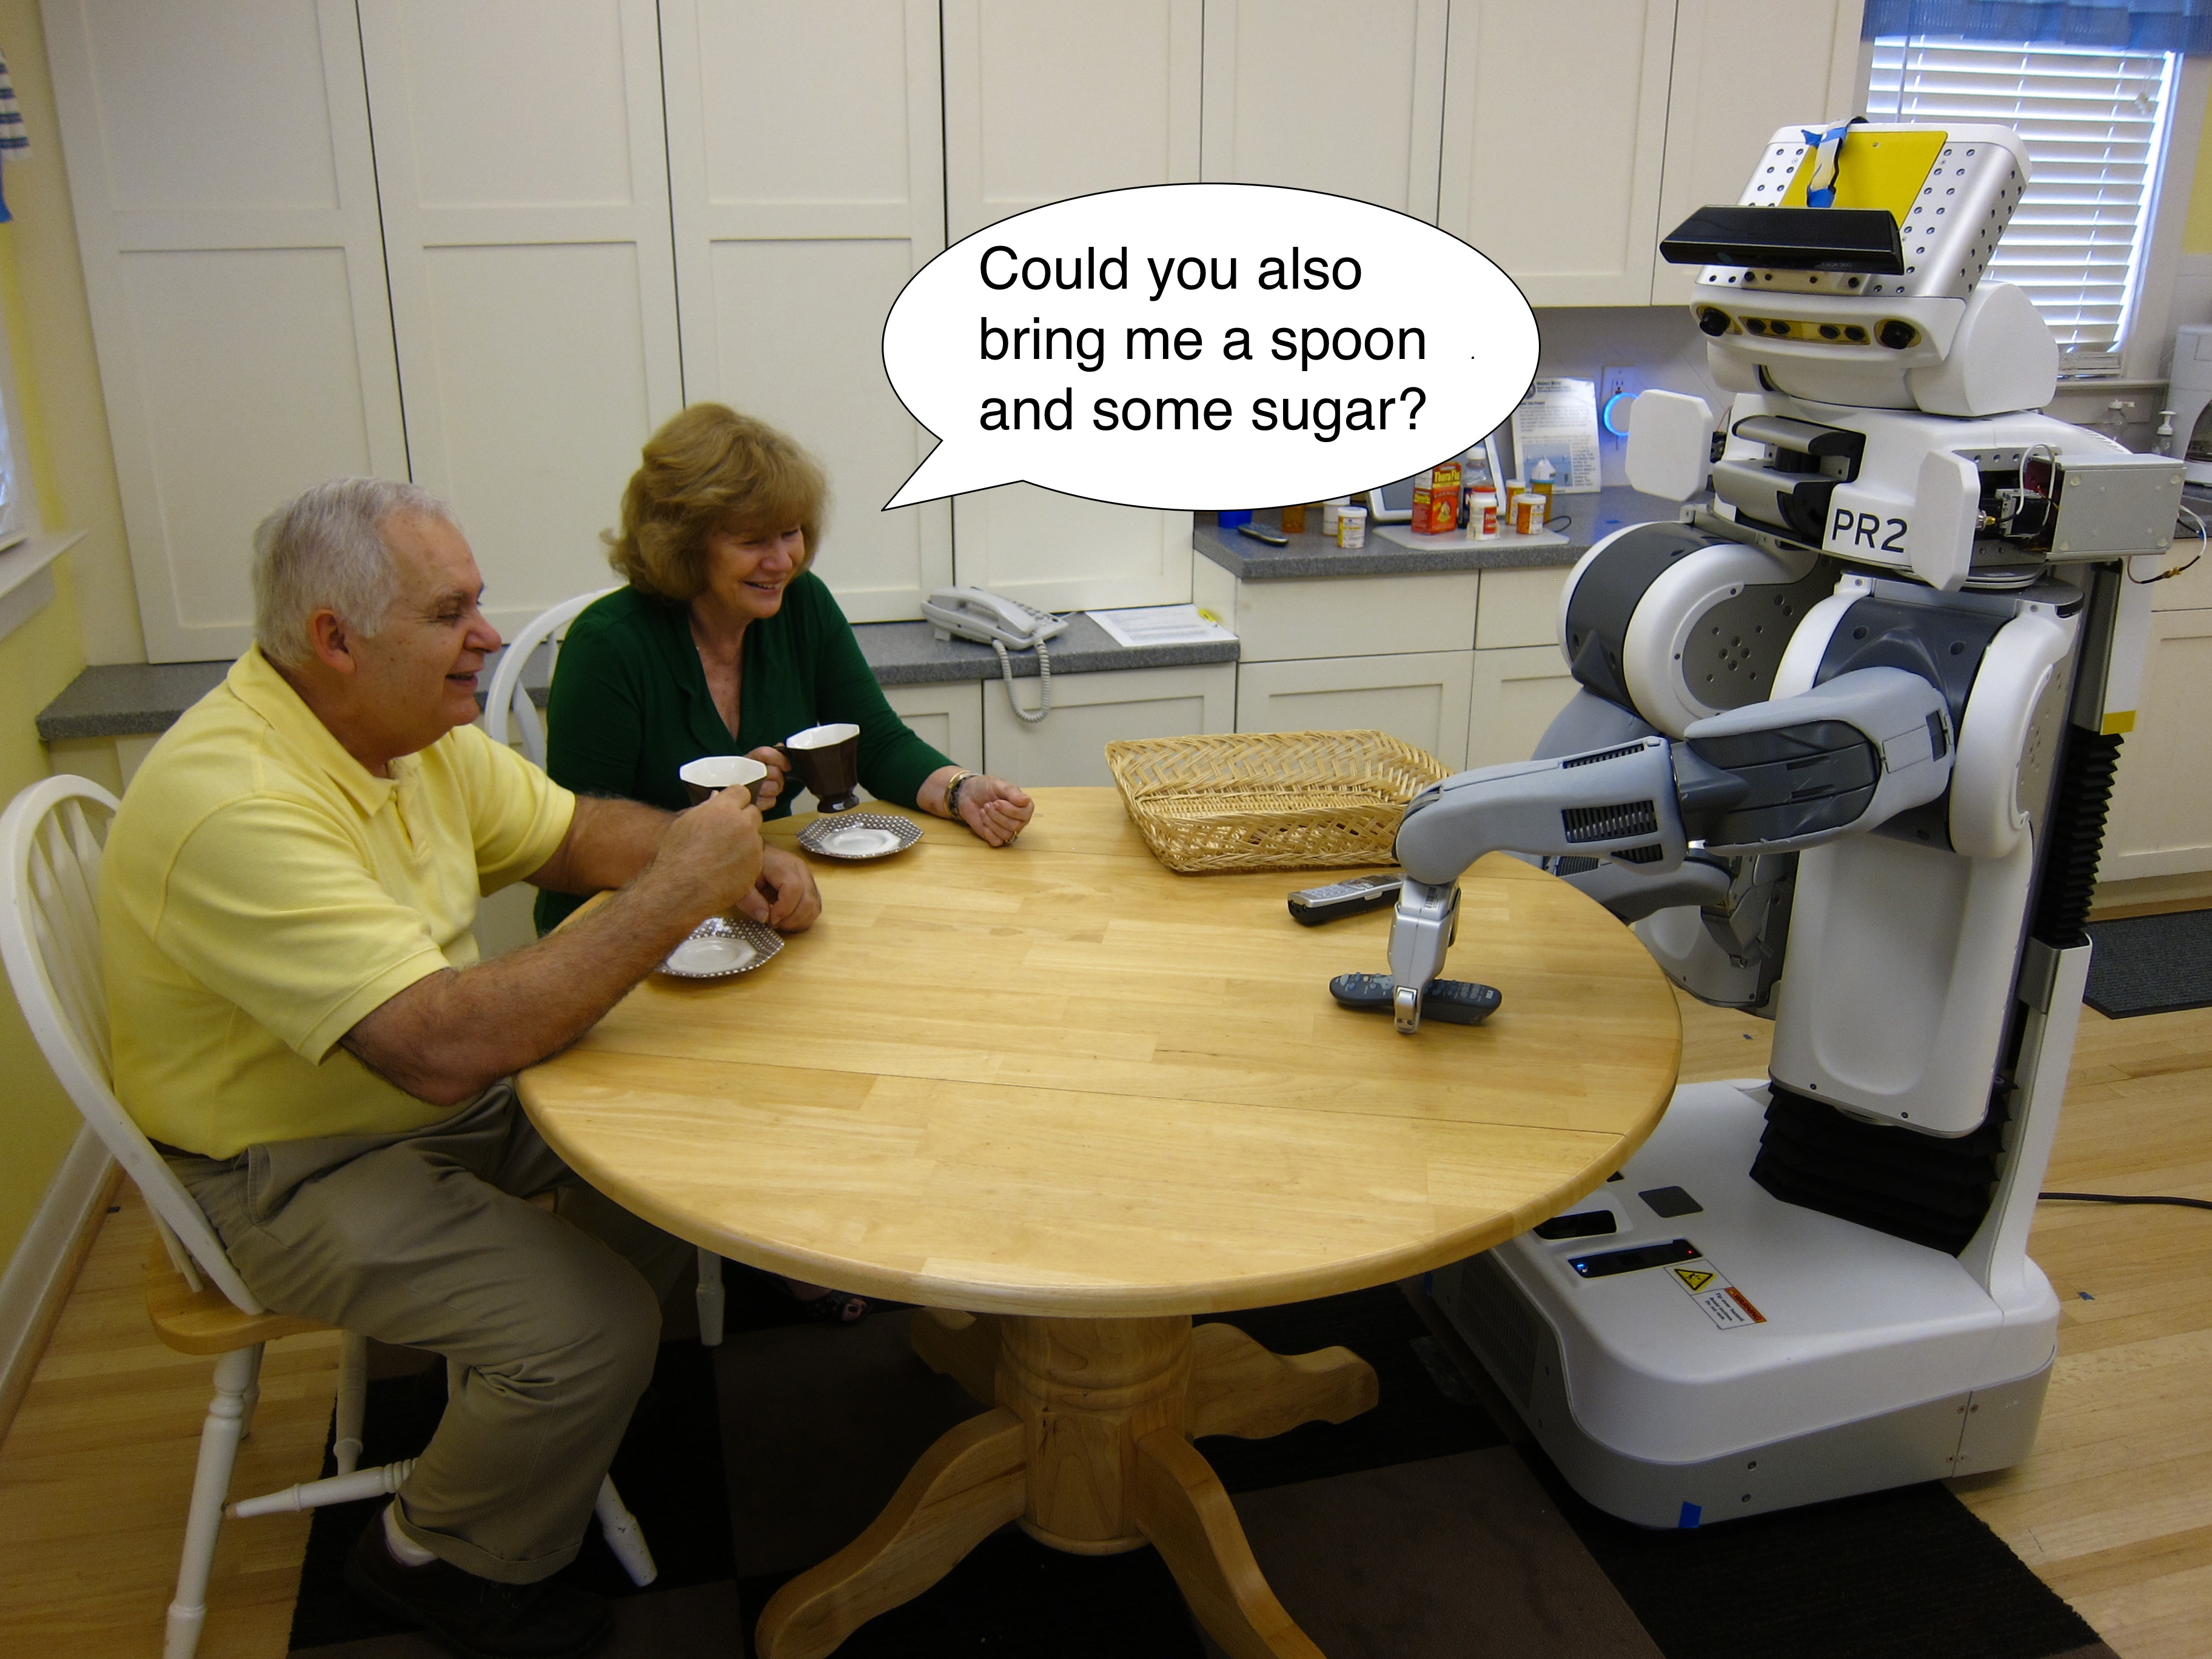
\includegraphics[width=3.2in]{img/robot_in_kitchen.jpg}

    \tiny{Original image courtesy of Wendy Rogers/Georgia Tech.}
  \end{center}
\end{frame}

\begin{frame}
  \frametitle{State of research}
\end{frame}

\begin{frame}
  \frametitle{Assumptions for the following treatment}
  \begin{itemize}
  \item There are no errors in the visual identification and classification of objects.
  \item The robot can successfully complete any movement and manipulation task,
    but motions take time, and are therefore expensive.
  \item The set of object types in the world is finite.
  \end{itemize}
\end{frame}

\begin{frame}
  \frametitle{Formulation of the problem}
  \begin{center}
    \vspace{-0.13in}
    Set of containers: $\{c_l\}$

    \spL[3-unknown-containers]

    Set of object types: $\{t_i\}$

    \spL[shape-universe-small]

    We want to find an object of type $q$ (the query type).

    \spL[blue-circle]

  \end{center}
\end{frame}

\begin{frame}
  \frametitle{Where is \spM[blue-circle]?}
  \begin{center}
    \spL[3-partially-observed-containers]

    \vspace{0.3in}

    Given that we have observed objects of types $\{t_{o_j}\}$ \\
    in container $c$, what is $\mathrm{P}(q \in c \, | \, \{t_{o_j}\})$ ?
  \end{center}
\end{frame}

